\documentclass[11pt]{article}

\usepackage{ulem}
\usepackage{tikz}
\usepackage{xurl}
\usepackage{float}
\usepackage{amsmath}
\usepackage{booktabs}
\usepackage{graphicx}
\usepackage{listings}
\usepackage[T5]{fontenc}
\usepackage{indentfirst}
\usepackage[utf8]{inputenc}
\usepackage[margin=1in]{geometry}
\usetikzlibrary{arrows.meta, positioning}

\begin{document}

\begin{center}

{\Large \textbf{UNIVERSITY OF SCIENCE AND TECHNOLOGY OF HANOI}}\\
\vspace{0.3cm}
----------------------o0o----------------------\\

\vspace{4cm}

{\large
\centerline{2540027 - Nguyễn Xuân Vinh}
}

\vspace{4cm}

{\Huge \textbf{BC3.04a Advanced Programming for HPC}}\\
\vspace{0.5cm}
Lecturer: Dr. Trần Giang Sơn

\vspace{4cm}

{\Large \textbf{REPORT LABWORK 6}}\\

\vspace{0.5cm}

{\large
Subjects: Map
}

\vspace{4cm}
\today
\end{center}

\newpage

\newpage

\tableofcontents

\newpage

\section{Objective}

The purpose of the labwork 6 is to implement image processing operations using a Map-style approach. The image is divided into smaller two-dimensional blocks, and the same operation is independently applied to each block.

Three image processing tasks were implemented:

\begin{itemize}
\item Grayscale image binarization.
\item Brightness control.
\item Blending two images.
\end{itemize}

Different 2D block sizes were also tested to compare their execution times.

\section{Implementation}

The input image was loaded from \texttt{/content/img.jpg} using OpenCV. The image has a size of $1080 \times 1920$ pixels with 3 color channels.

The main function used for the Map-style processing is \texttt{map\_2d()}. It divides the input image into blocks according to the specified block size. For every block, an operation is applied independently, and the processed blocks are then placed into the corresponding positions of the output image.

The general processing flow is:

\begin{center}
Input Image $\rightarrow$ 2D Blocks $\rightarrow$ Map Operation $\rightarrow$ Output Image
\end{center}

The block size can be changed through the \texttt{BLOCK\_SIZE} parameter.

\section{6a - Grayscale Image Binarization}

First, the color image is converted from BGR to grayscale. For each pixel, the grayscale value is calculated using:

$$
Gray = 0.114B + 0.587G + 0.299R
$$

The grayscale operation is applied independently to every 2D block using \texttt{map\_2d()}.

After obtaining the grayscale image, binarization is performed using a threshold value of 128:

$$
Binary(x,y) =
\begin{cases}
255, & Gray(x,y) \geq 128\\
0, & Gray(x,y) < 128
\end{cases}
$$

The binarization operation is also applied block by block.

\begin{figure}[H]
\centering
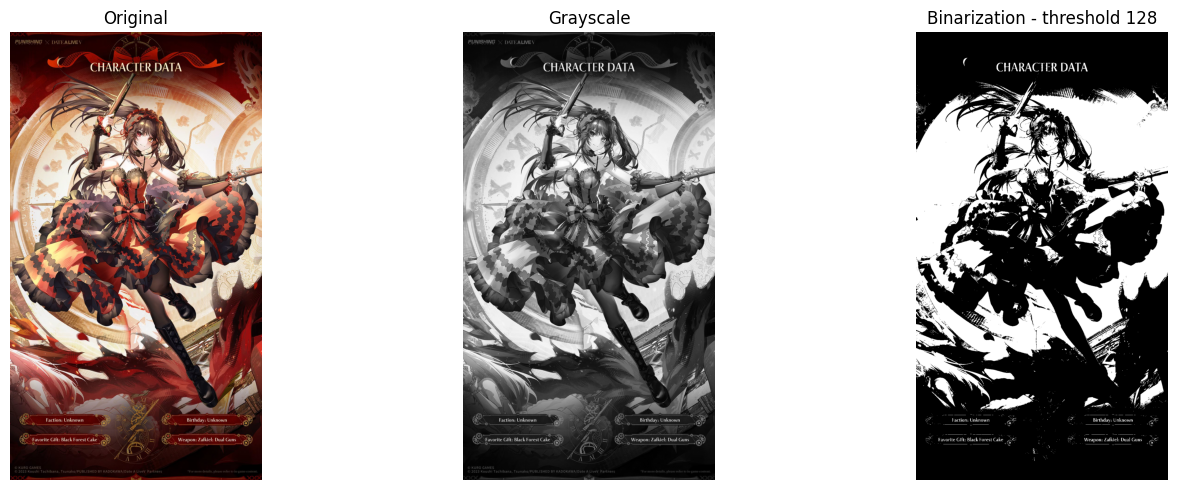
\includegraphics[width=0.95\textwidth]{6a_results.png}
\caption{Results of grayscale conversion and image binarization.}
\label{fig:6a}
\end{figure}

\section{6b - Brightness Control}

For brightness control, a value of 50 was used. The operation is applied independently to every image block.

For increasing brightness:

$$
I_{bright} = \operatorname{clip}(I + 50, 0, 255)
$$

For decreasing brightness:

$$
I_{dark} = \operatorname{clip}(I - 50, 0, 255)
$$

The clipping operation keeps the pixel values in the valid range from 0 to 255.

The operations were implemented using the \texttt{brightness\_operation()} and \texttt{darkening\_operation()} functions.

\begin{figure}[H]
\centering
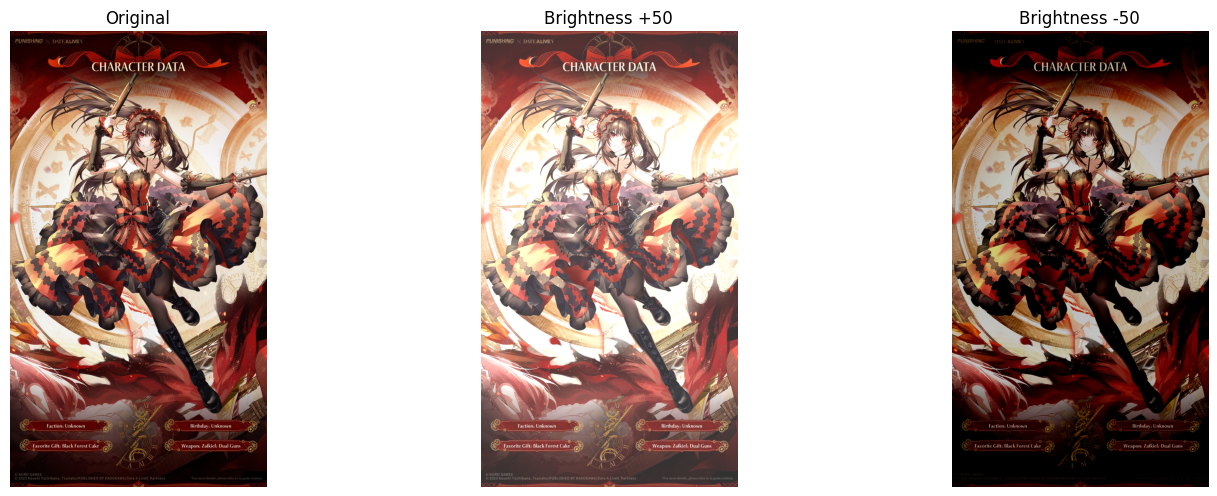
\includegraphics[width=0.95\textwidth]{6b_results.png}
\caption{Results of brightness increase and brightness decrease.}
\label{fig:6b}
\end{figure}

\section{6c - Blending Two Images}

For blending, two images with the same dimensions are required. Since only one input image was provided, a second image was created by horizontally flipping the original image:

\begin{verbatim}
image2 = cv2.flip(image, 1)
\end{verbatim}

The two images are divided into corresponding 2D blocks and each pair of blocks is blended independently.

The blending formula is:

$$
C = \alpha A + (1-\alpha)B
$$

where $A$ is a block from the first image, $B$ is the corresponding block from the second image, and $\alpha$ is the blending coefficient.

In this experiment:

$$
\alpha = 0.5
$$

Therefore, both images contribute equally to the resulting image.

\begin{figure}[H]
\centering
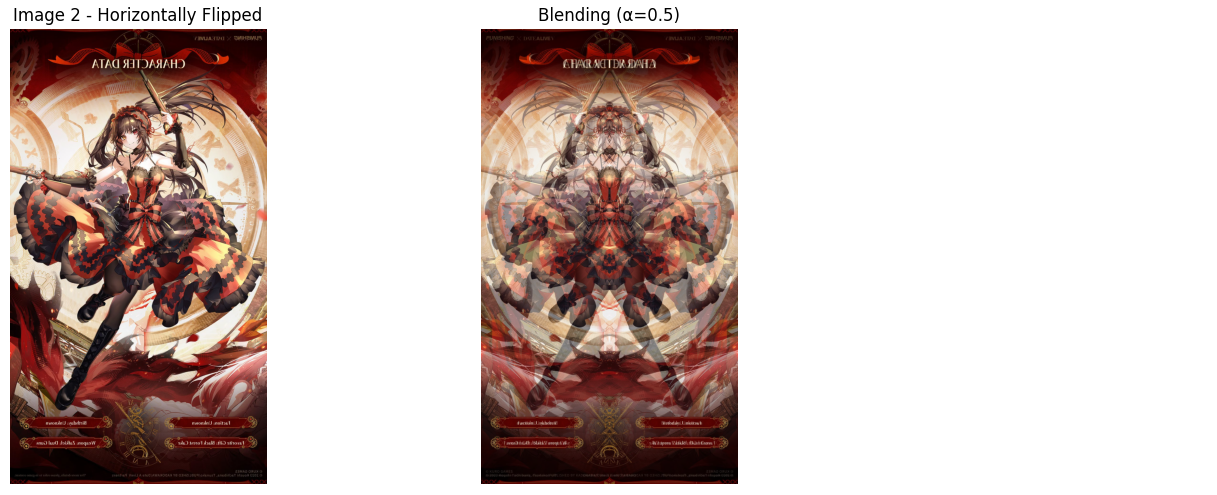
\includegraphics[width=0.95\textwidth]{6c_results.png}
\caption{Results of image flipping and blending with $\alpha=0.5$.}
\label{fig:6c}
\end{figure}

\section{Experiment with Different Block Sizes}

Five different 2D block sizes were tested:

$$
4\times4,\quad
8\times8,\quad
16\times16,\quad
32\times32,\quad
64\times64
$$

The execution time of binarization, brightness control, and blending was measured for each block size.

\begin{table}[H]
\centering
\caption{Execution time for different 2D block sizes}
\label{tab:benchmark}
\begin{tabular}{cccc}
\toprule
Block Size & Binarization (s) & Brightness (s) & Blending (s) \\
\midrule
$4\times4$   & 3.967172 & 1.313303 & 1.446491 \\
$8\times8$   & 0.696770 & 0.333042 & 0.382678 \\
$16\times16$ & 0.194444 & 0.098090 & 0.125163 \\
$32\times32$ & 0.067388 & 0.029771 & 0.043326 \\
$64\times64$ & 0.028008 & 0.010484 & 0.020513 \\
\bottomrule
\end{tabular}
\end{table}

The results for the different block sizes were also generated visually for each of the three operations.

\begin{figure}[H]
\centering
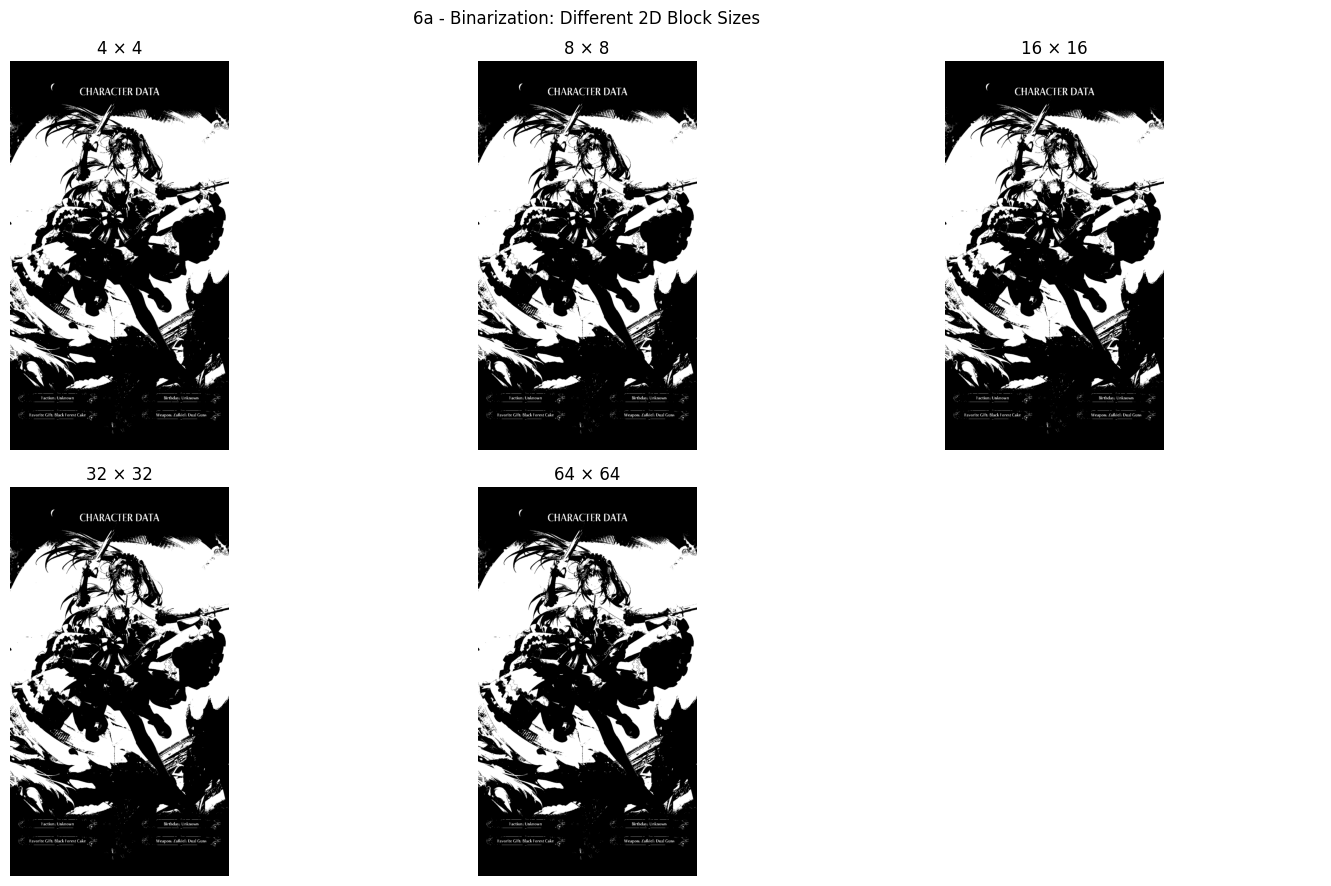
\includegraphics[width=0.95\textwidth]{6a_block_sizes.png}
\caption{Binarization results using different 2D block sizes.}
\label{fig:6a_blocks}
\end{figure}

\begin{figure}[H]
\centering
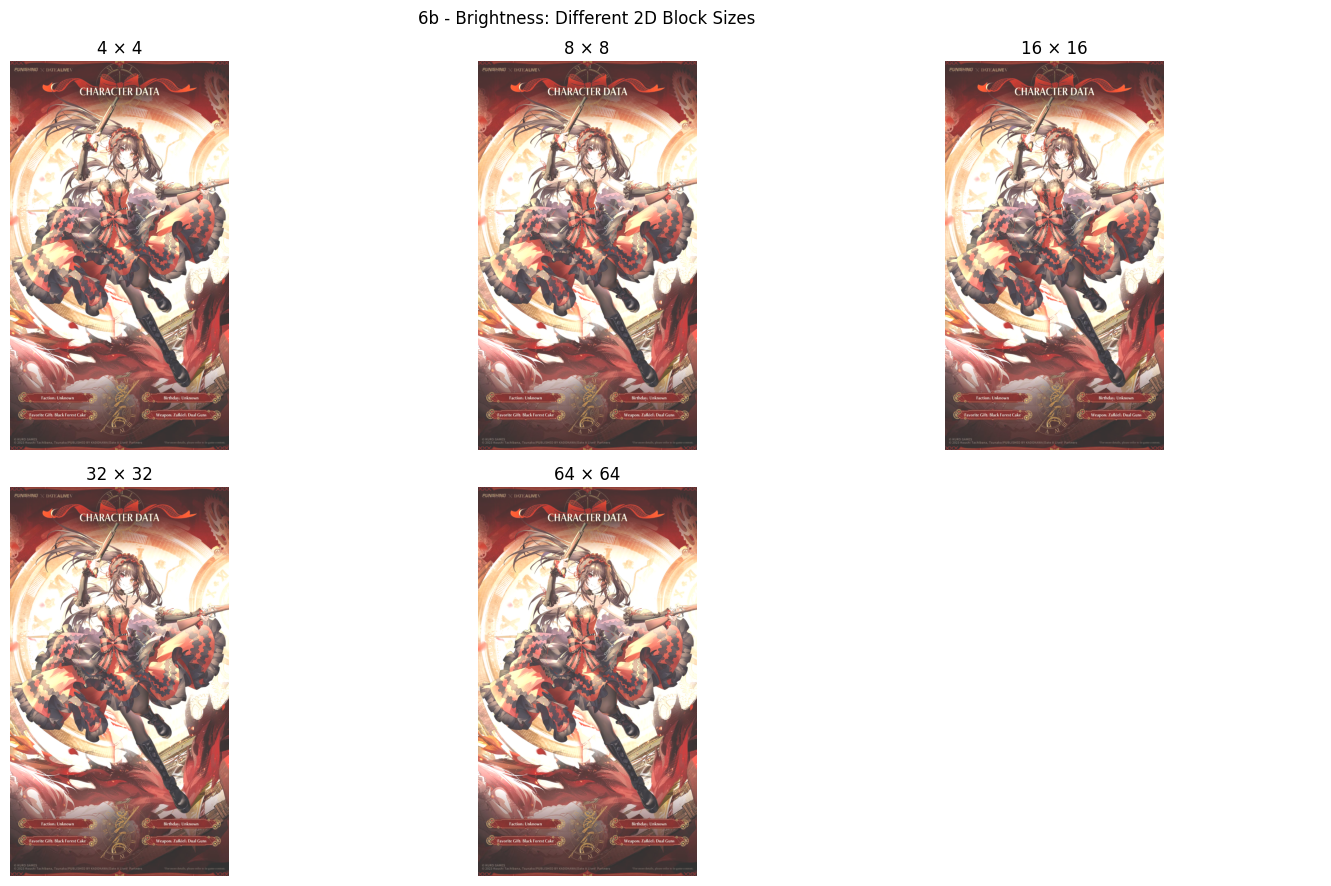
\includegraphics[width=0.95\textwidth]{6b_block_sizes.png}
\caption{Brightness results using different 2D block sizes.}
\label{fig:6b_blocks}
\end{figure}

\begin{figure}[H]
\centering
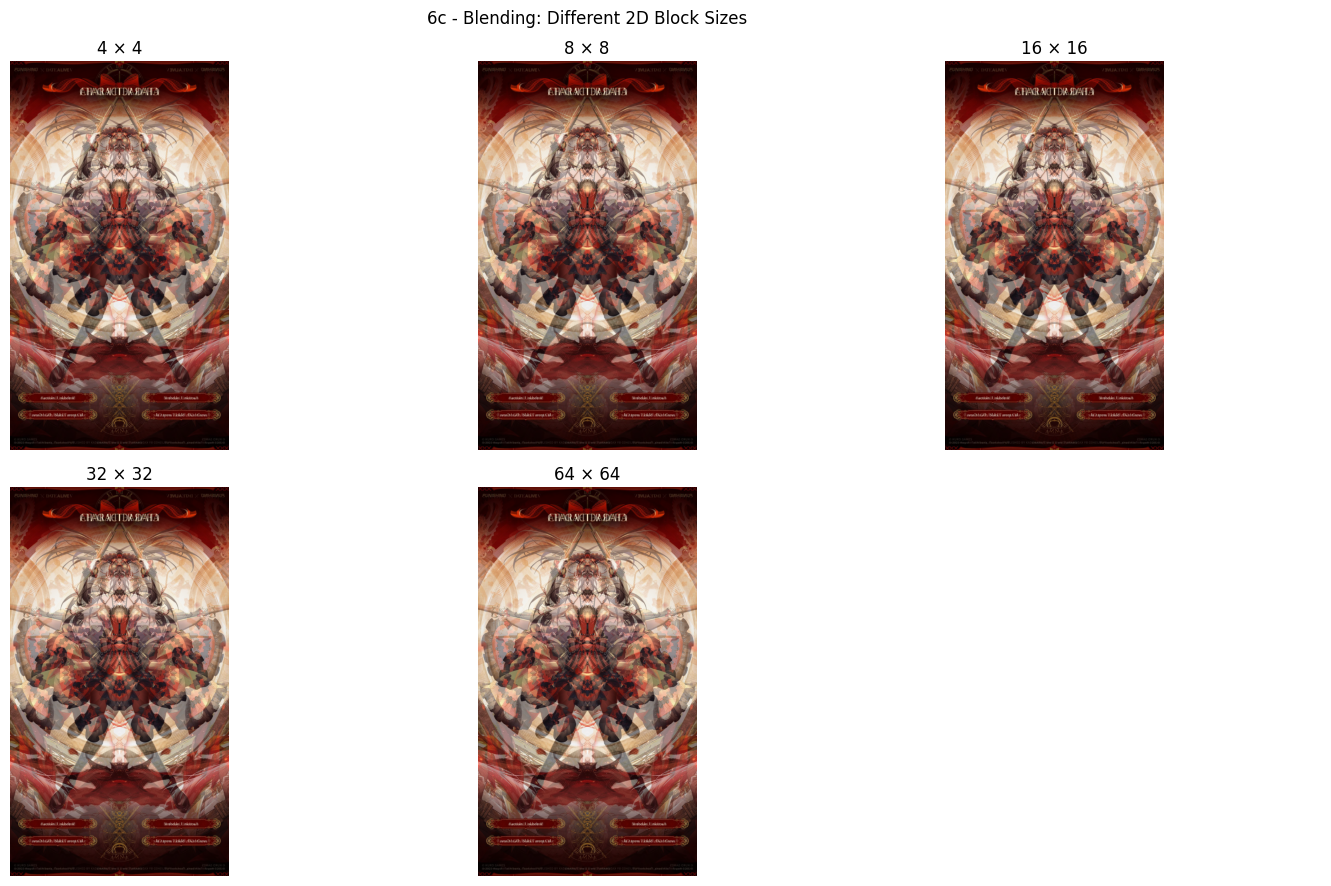
\includegraphics[width=0.95\textwidth]{6c_block_sizes.png}
\caption{Blending results using different 2D block sizes.}
\label{fig:6c_blocks}
\end{figure}

\section{Conclusion}

In this labwork, three image processing operations were implemented using a 2D Map-style approach. The \texttt{map\_2d()} function divides the image into blocks and applies the corresponding operation independently to each block.

The implemented operations were grayscale binarization, brightness control, and image blending. Different block sizes from $4\times4$ to $64\times64$ were also tested.

For the tested implementation, the execution time decreased as the block size increased. The $64\times64$ block size had the lowest measured execution time for all three operations in this experiment.

\end{document}